\section{Method:Digital back propagation}
This section aims to design the digital back propagation algorithm (See (\ref{DBP})). We concentrate on the central channel $A_0(z,t)$.
$$
DBP: A_0(L,t) \rightarrow \hat{A}_0(t)  
$$
The main challege is that we can not get the information of other channels. So we can not implement full channel digital propagation (FDBP).
We can construct several digital compensation method:

\subsection{Dispersion only DBP (DO-DBP)}
This method only compensate the linear distortion.
$$
\hat{A_0}(0) = L_{H_0(-L)}(A_0(L))
$$
\begin{figure}[htbp]
\centering
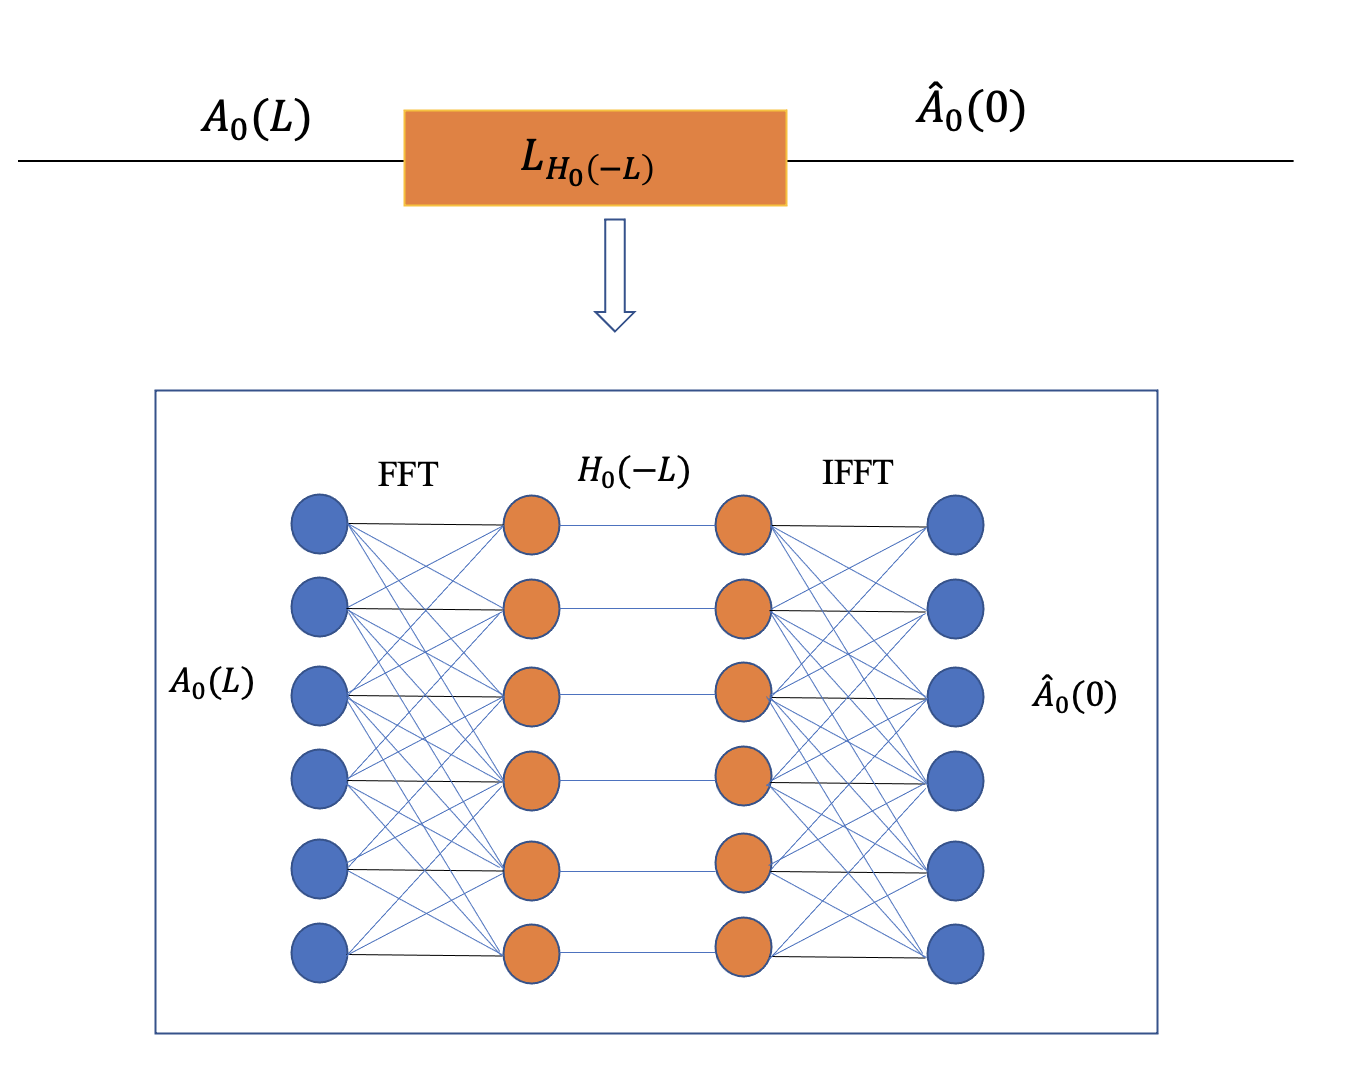
\includegraphics[width=0.6\linewidth]{img/DO-DBP.png}
\caption{Dispersion Only DBP}
\label{DO-DBP}
\end{figure}
\subsection{Single channel DBP (SC-DBP)}
$$
\hat{A}_0(0) = \left(\prod_{i=1}^{K} NL_{-dz,S_0=0} \circ L_{H_0(-dz)}\right)A_0(L,t)
$$
where K is $L/dz$ the span numbers. 
\begin{figure}[htbp]
  \centering
  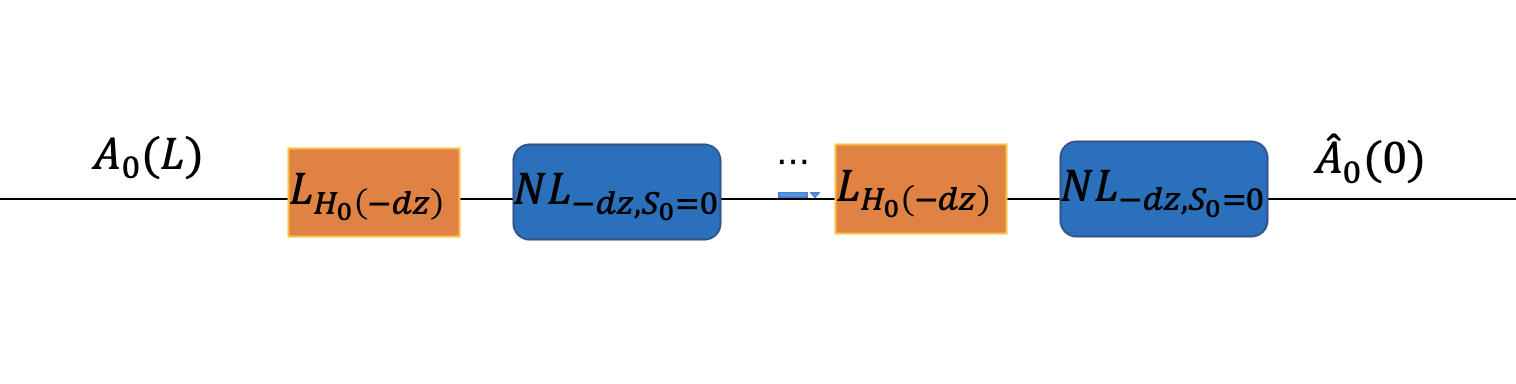
\includegraphics[width=0.6\linewidth]{img/SC-DBP.png}
  \caption{Single Channel DBP}
  \label{SC-DBP}
\end{figure}

\subsection{Neural Network DBP (NN-DBP)}
Notice that (\ref{linear step}) is a linear transform and (\ref{nonlinear step}) is a 
point wise nonlinear transform. SSFM are composed with Linear transform and nonlinear activations just like deep neural 
network.\cite{hager2020} and \cite{fan2020NC} find this similiar structure 
between SSFM and DNN. Set some parameters in SSFM to free then get NN-DBP. 
\begin{figure}[htbp]
\centering
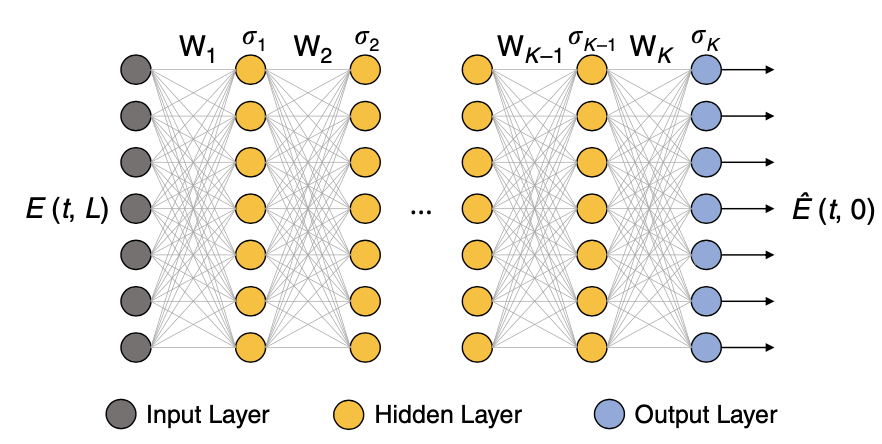
\includegraphics[width=0.6\linewidth]{img/NN.png}
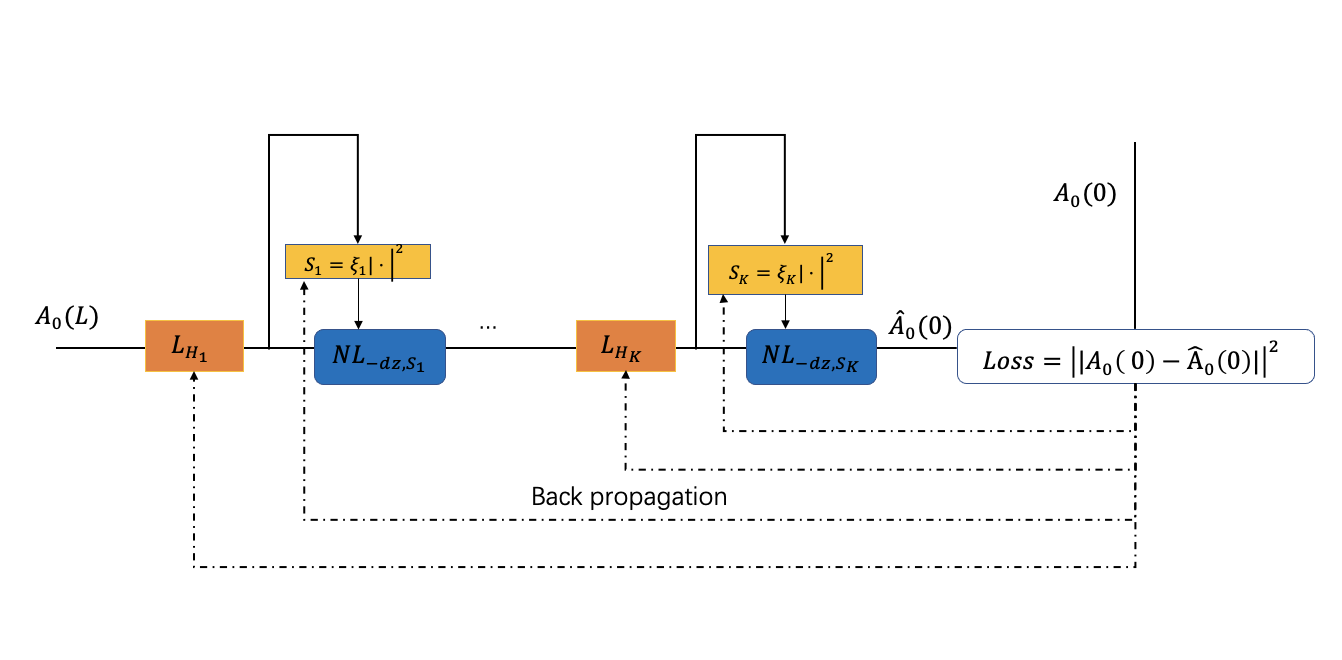
\includegraphics[width=0.6\linewidth]{img/NN-DBP.png}
\caption{NN structure \cite{fan2020NC}}
\label{NN}
\end{figure}
$$
D_i(u) = NL_{-dz,S_0 = \xi_i |u|^2} \circ L_{H_i}
$$
$$
\hat{A}(0) = \left(\prod_{i=1}^{K} D_i\right)A_0(L)
$$
where $\{\xi_i,H_i\}$ is the trained parameters.

$$
loss = \sum_{a_k^i \sim Uniform(\mathcal{X})} \|\hat{A}(0,t) - A(0,t)\|^2
$$

\subsection{Meta-1 DBP}
Use two fully connected networks to estimate $S_0$ and $H_0$ in each step. We want to guess some information
 from $A_0(L)$. This is a meta neural network.
\begin{equation}
S_0 = \phi(u,\theta_i), H_0 = \psi(u,\mu_i)
\end{equation}
$$
D_i(u) = \left(NL_{-dz,S_0=\phi(u;\theta_i)} \circ L_{H_0=\psi(u;\mu_i)}\right) (u)
$$

$$
\hat{A}(0,t) = \left(\prod_{i=1}^{K} D_i\right)A_0(L,t)
$$

where $\phi$ and $\psi$ is two fully connected networks, $\{\theta_i,\mu_i\}$ is the trained parameter. 

$$
loss = \sum_{a_k^i \sim Uniform(\mathcal{X})} \|\hat{A}(0,t) - A(0,t)\|^2
$$
\begin{figure}[htbp]
\centering
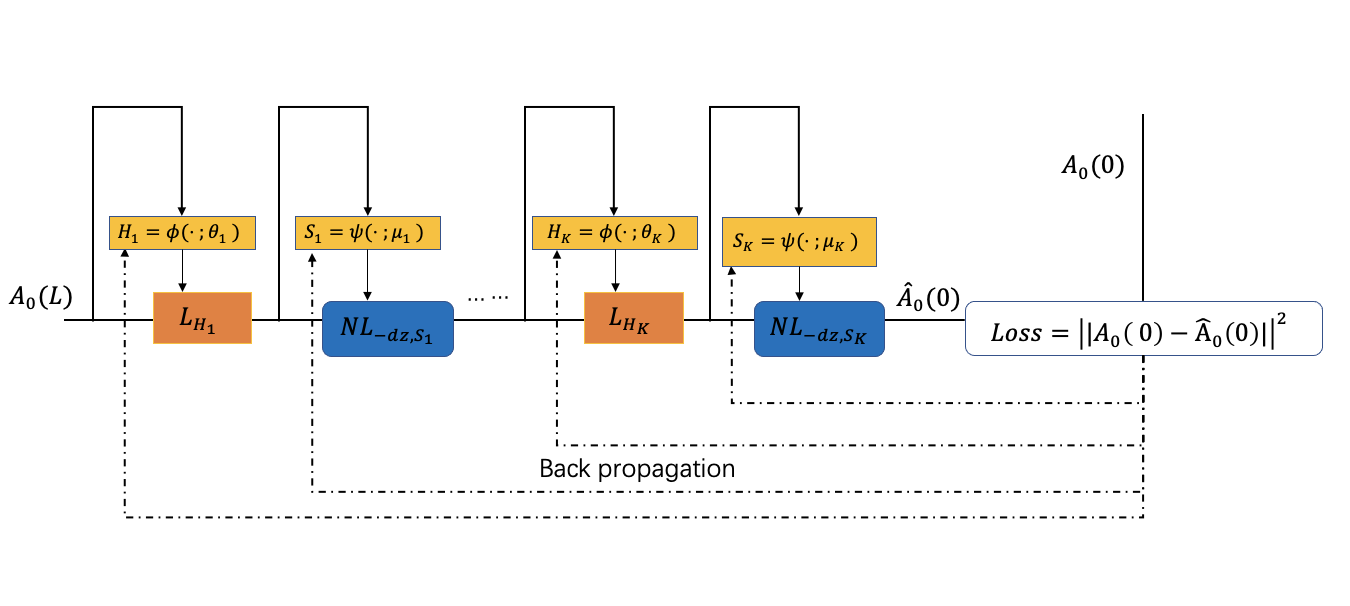
\includegraphics[width=0.6\linewidth]{img/Meta-1.png}
\caption{Meta-1 DBP structure}
\label{Meta-1}
\end{figure}

\begin{figure}[htbp]
  \centering
  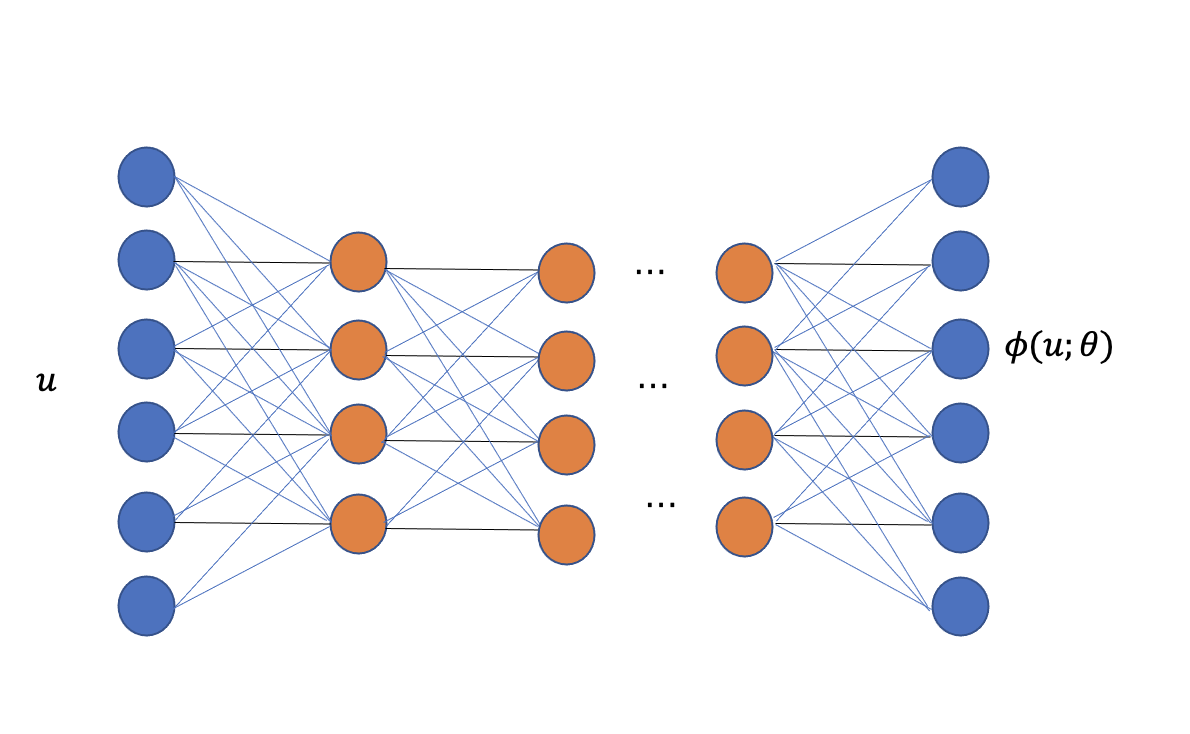
\includegraphics[width=0.4\linewidth]{img/FNNphi.png}
  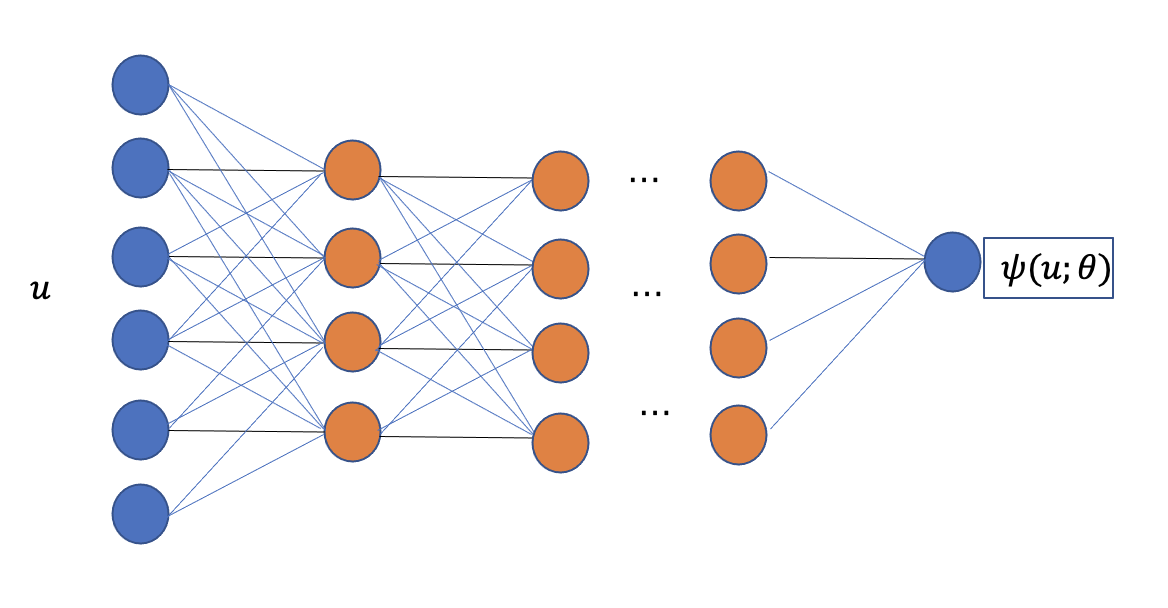
\includegraphics[width=0.4\linewidth]{img/FNNpsi.png}
  \caption{FNN structure}
  \label{FNN1}
  \end{figure}

\newpage
\subsection{Meta-2 DBP}
\begin{equation}
  S_0 = \phi(u,\theta_i)|u|^2, H_0 = \psi(u,\mu_i)
  \end{equation}
Change the meta form.
$$
D_i(u) = \left(NL_{-dz,S=\phi(u;\theta_i)|u|^2} \circ L_{-dz,H=\psi(u;\mu_i)}\right) (u)
$$

$$
\hat{A}(0,t) = \left(\prod_{i=1}^{K} D_i\right)A_0(L,t)
$$

where $\phi$ and $\psi$ is two fully connected networks, $\{\theta_i,\mu_i\}$ is the trained parameter. 

$$
loss = \sum_{a_k^i \sim Uniform(\mathcal{X})} \|\hat{A}(0,t) - A(0,t)\|^2
$$

\subsection{Meta-3 DBP}
Share the meta-net weight in different steps.
$$
D(u) = \left(NL_{-dz,S=\phi(u;\theta)} \circ L_{-dz,H=\psi(u;\mu)}\right) (u)
$$

$$
\hat{A}(0,t) = \left(\prod_{i=1}^{K} D_i\right)A_0(L,t)
$$

where $\phi$ and $\psi$ is two fully connected networks, $\{\theta,\mu\}$ is the trained parameter. 

$$
loss = \sum_{a_k^i \sim Uniform(\mathcal{X})} \|\hat{A}(0,t) - A(0,t)\|^2
$$

\section{Experiments result}
The details of experiment are showed in Table \ref{ex details}. We construct two training data sets.
\begin{enumerate}
  \item Data set A: $P_i = 50 [mW]$.
  \item Date set B: $P_i$ is i.i.d sampled from Uniform([50 mW,60 mW]) in each epoch.
\end{enumerate}
We use different widths and depths for A and B. See Table \ref{NN setting}. The loss curves are shown
in Figure \ref{loss}. Under setting A, we can see Meta-1 to Meta-3 can achive
better minimizers than NN-DBP. These methods converge steadily. Under Setting B, training becomes untractable.
The costellations are shown in Figure \ref{A fig} and \ref{B fig}. The BER results are shown in Table \ref{A table} and Table \ref{B table}.
We mainly consider comparation of 4 methods: NN-DBP,Meta-1,Meta-2,Meta-3.We can get conclusions as follows:
\begin{enumerate}
\item Under setting A:
\begin{itemize}
\item From the loss curve \ref{loss}, the four methods all converge smoothly, and the convergence point from Meta-1 to Meta-3 is better than NN-DBP. 
The loss curves of Meta-1 and Meta-2 almost overlap, which also shows a certain equivalence of the two methods. Meta-3 converges faster than Meta-1 and Meta-2, 
but the minimum point reached in the end is not as good as the first two.
\item From the costellation diagram \ref{A fig},when the test power is equal to the training power, the four methods all show the best results.When the test 
power is not equal to the training power, the non-linear phase shift is not perfectly compensated. Compared with the ideal result, there is a phase deflection overall
\item From table \ref{A table},when the test power is equal to 50mW, Meta-1 to Meta-3 are better than NN-DBP by about $2\%$. 
Other test power performances are not good, and there is no comparative value.
没有比较价值。
\end{itemize}
\item Under setting B:(Since Meta-1 and Meta-2 behave very similarly in A, the Meta-2 experiment was omitted here.)
\begin{itemize}
\item From the loss curve \ref{loss}, the convergence of the four methods is very difficult. Meta-1 is better than Meta-3. Meta-3 is better than NN-DBP
\item From the constellation diagram, when test power = 55mW, the four methods perform best. Other power values behave similarly to A, with a phase rotation difference overall. This means neural network
Learned an average power result in the training set. This also shows that our method is invalid without knowing the power of the interfering channel
\item From table \ref{A table},when the test power is equal to 55 mW, Meta-1 and Meta-3 are better than NN-DBP by about $2\%$. 
Other test power performances are not good, and there is no comparative value.
\end{itemize}
\end{enumerate}

\begin{table}[htbp]
  \centering
  \begin{tabular}{lll}
    \hline
    setting       & width & depth \\
    \hline
    A           &  60   &   2   \\
    \hline
    B           &  120  &   3   \\
    \hline
  \end{tabular}
  \caption{experiments details}
  \label{NN setting}
\end{table}

\begin{table}[htbp]
  \centering
  \begin{tabular}{llll}
  parameter        & variable  & quantity & unit \\
  \hline
  attenuation      & $\alpha$  &   0.2     &  [dB/km]  \\
  \hline
  dispersion       & $\beta_2$ &   -21.68  &   [$ps^2 km^{-1}$]   \\
  \hline
  nonlinear        & $\gamma$  &   1.37   &  [$W^{-1} km^{-1}$]   \\
  \hline
  peak power       & $P_0$     &   50     &  [mW] \\
  \hline
  number of WDM channel& $2M+1$  &    3   &   1 \\
  \hline
  length of fiber  & L         &     100   & [km] \\
  \hline
  symbol rate      & $R_s = \frac{1}{T_f}$ & 10 & [GHz]\\
  \hline
  central wavelength & $\lambda_0$ & 1550  & [nm] \\
  \hline
  channel space      &   $\Delta \lambda $     & 0.4   & [nm] \\
  \hline 
  roll              & $\beta$     & 0.2 & 1 \\
  \hline
  noise level       & $\sigma$    & 0.002 & 1 \\
  \hline
  number of symbols  & N          & 128   & 1 \\
  \hline
  number of samples/symbol & $N_t$ & 8    & 1 \\
  \hline
  \end{tabular}
  \caption{experiments details}
  \label{ex details}
\end{table}


\begin{figure}[htbp]
  \centering
  \subfigure[Loss curve for Data set A]{
    \begin{minipage}[t]{0.4\linewidth}
      \centering
      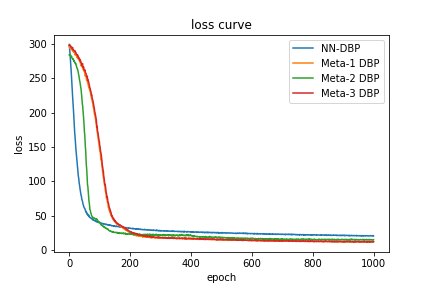
\includegraphics[width=0.9\linewidth]{img/expriment/fixpower_loss.png}
    \end{minipage}
  }
  \subfigure[Loss curve for Data set B]{
    \begin{minipage}[t]{0.4\linewidth}
      \centering
      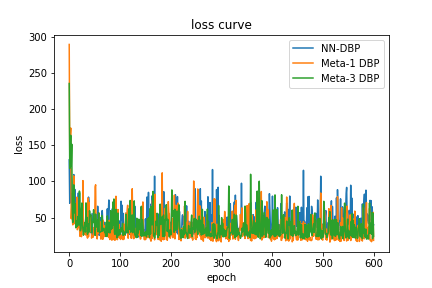
\includegraphics[width=0.9\linewidth]{img/expriment/W120-D3-loss.png}
    \end{minipage}
  }
  \caption{Loss curve for Data set A and B}
  \label{loss}
  \end{figure}


  
  \begin{figure}[htbp]
  \centering
  \subfigure[test power: 50mW]{
    \begin{minipage}[t]{0.8\linewidth}
      \centering
      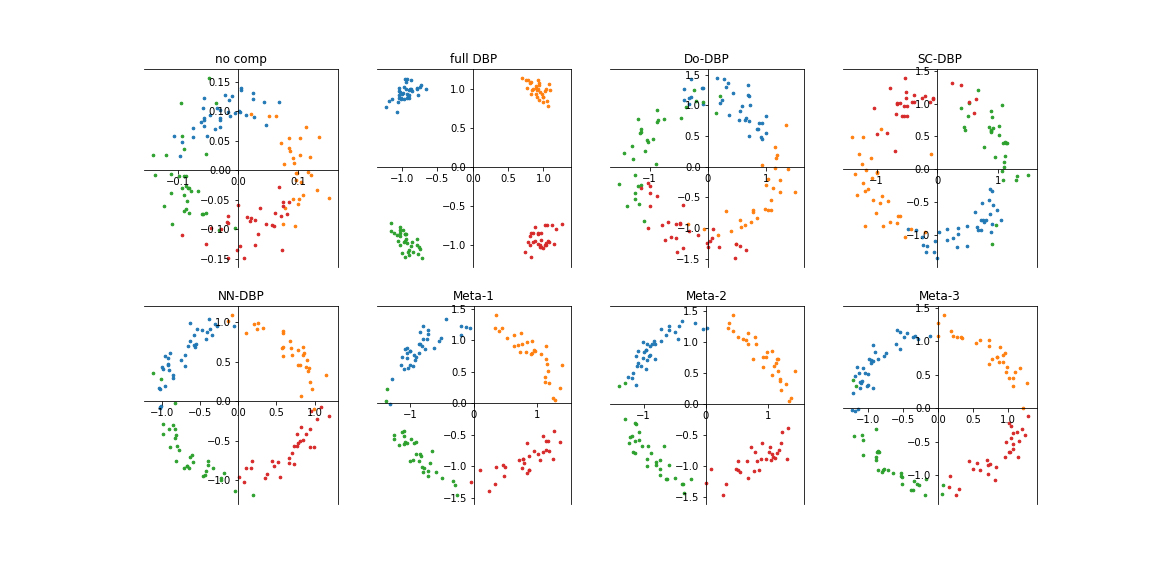
\includegraphics[width=1\linewidth]{img/expriment/W60-D2-P50star.png}
    \end{minipage}
  }
  
  \subfigure[test power: 55 mW]{
    \begin{minipage}[t]{0.8\linewidth}
      \centering
      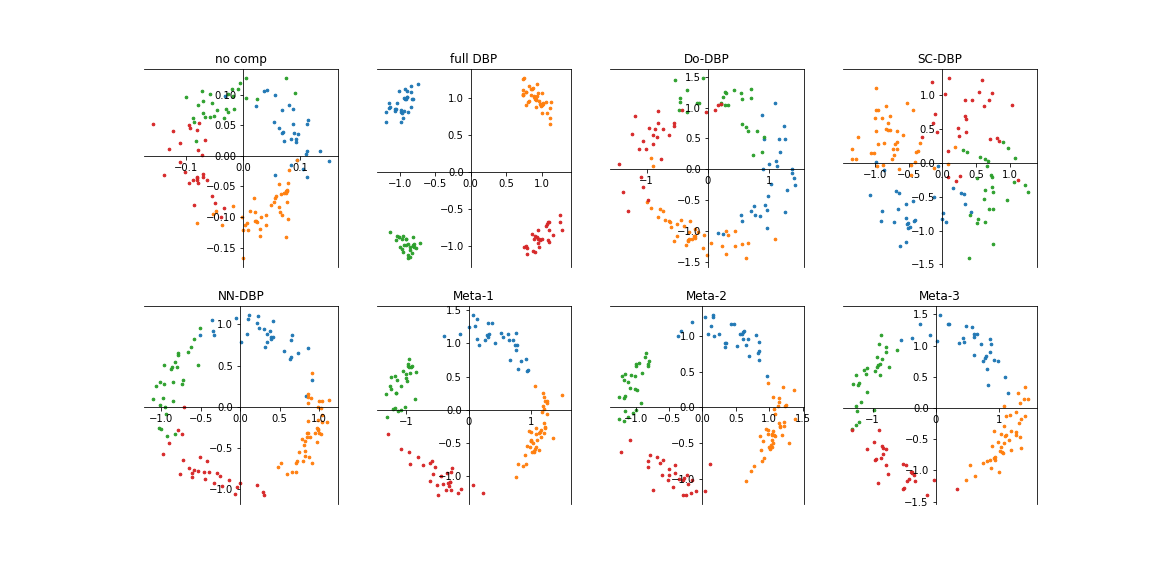
\includegraphics[width=1\linewidth]{img/expriment/W60-D2-P55star.png}
    \end{minipage}
  }
  
  \subfigure[test power: 45 mW]{
    \begin{minipage}[t]{0.8\linewidth}
      \centering
      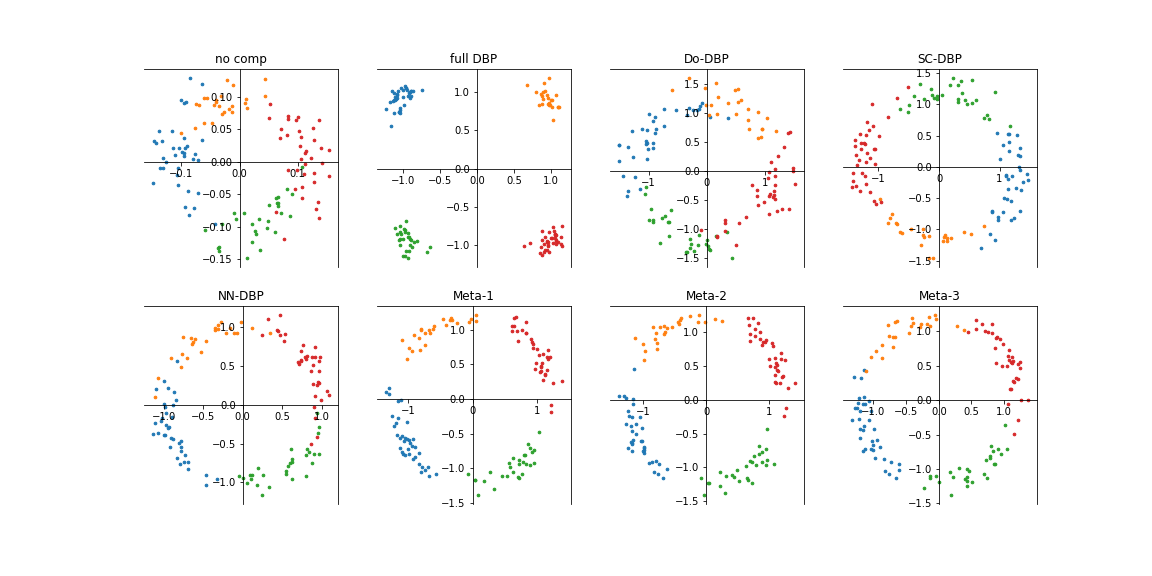
\includegraphics[width=1\linewidth]{img/expriment/W60-D2-P45star.png}
    \end{minipage}
  }
  \caption{Plot the $\tilde{x}_k^0$. Training with Data Set A.  Test with power: 50[mW],52[mW], 45[mW]}
  \label{A fig}
  \end{figure}


\begin{table}[htbp]
\centering
\begin{tabular}{llll}
\hline
\multicolumn{2}{l}{Test power: 50[mW]} & Test power: 52[mW] & Test power: 45[mW] \\
\hline
Method & Acc(100 times mean)  & Acc(100 times mean)  & Acc(100 times mean)\\
    DO-DBP  &  0.586914   &    0.421367  &    0.9275  \\
    SC-DBP  &  0.0989844  &   0.216875  &   0.12375 \\
    NN-DBP  &  0.963242   &   0.886992  &   0.573984 \\
    Meta-1  &  0.989297   &   0.910117   &   0.559688 \\
    Meta-2  &  0.984766   &   0.895469   &   0.556758 \\
    Meta-3  &  0.975234   &   0.893203 &   0.589961 \\
    \hline
\end{tabular}
\caption{Test result. Training data: A}
\label{A table}
\end{table}

\begin{table}[htbp]
  \centering
  \begin{tabular}{ll}
  \hline
  \multicolumn{2}{l}{Test power: 50[mW]}\\
  Method    &    BER    \\
   no comp  &   0.518125 \\
  full DBP  &   0 \\
    DO-DBP  &   0.334219 \\
    SC-DBP  &   0.381836 \\
    NN-DBP  &   3.08594e-05 \\
    Meta-1  &   2.73437e-06 \\
    Meta-2  &   1.5625e-06 \\
    Meta-3  &   1.01563e-05 \\
      \hline
  \end{tabular}
  \caption{TEST}
  \label{test test}
  \end{table}

\begin{table}[htbp]
  \centering
  \begin{tabular}{llll}
  \hline
  \multicolumn{2}{l}{Test power: 50[mW]} & Test power: 55[mW] & Test power: 60[mW] \\
  \hline
  Method & Acc(100 times mean)   & Acc(100 times mean)  & Acc(100 times mean)\\
      DO-DBP  &  0.587461  &   0.170586  &   0.318281 \\
      SC-DBP  &   0.0934766  &   0.410273  &    0.652031 \\
      NN-DBP  &   0.594141 &   0.948281  &   0.635977\\
      Meta-1  & 0.600195 &    0.974766  &    0.606836\\
      Meta-3  &  0.603828  &    0.964063  &   0.601992 \\
      \hline
  \end{tabular}
  \caption{Test result. Training data: B}
  \label{B table}
  \end{table}

\begin{figure}[htbp]
\centering
\subfigure[test power: 50mW]{
  \begin{minipage}[t]{0.8\linewidth}
    \centering
    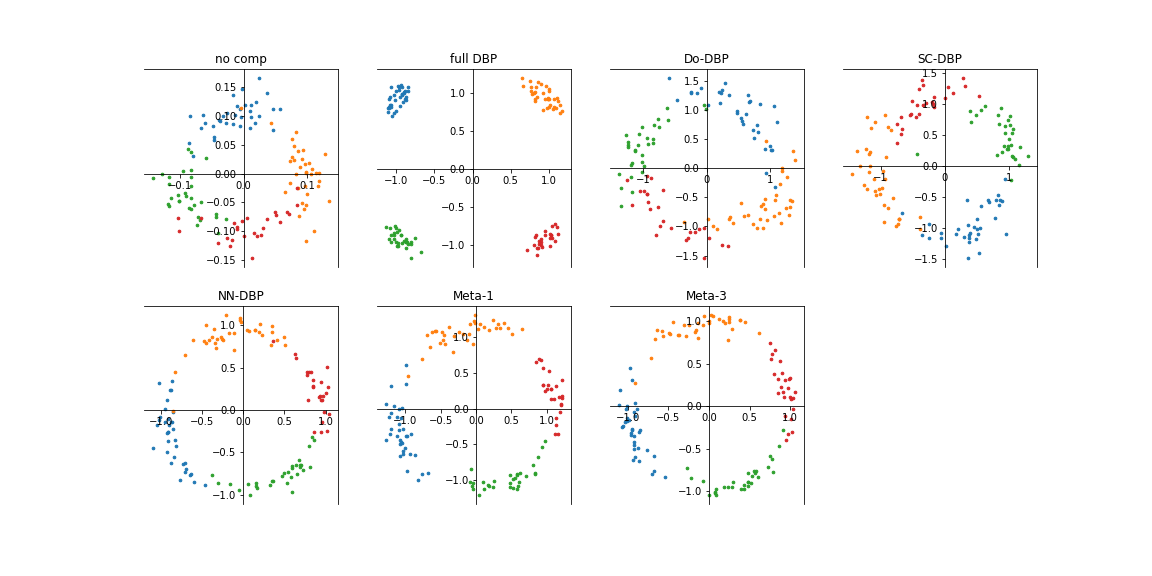
\includegraphics[width=1\linewidth]{img/expriment/W120-D3-P50star.png}
  \end{minipage}
}

\subfigure[test power: 55 mW]{
  \begin{minipage}[t]{0.8\linewidth}
    \centering
    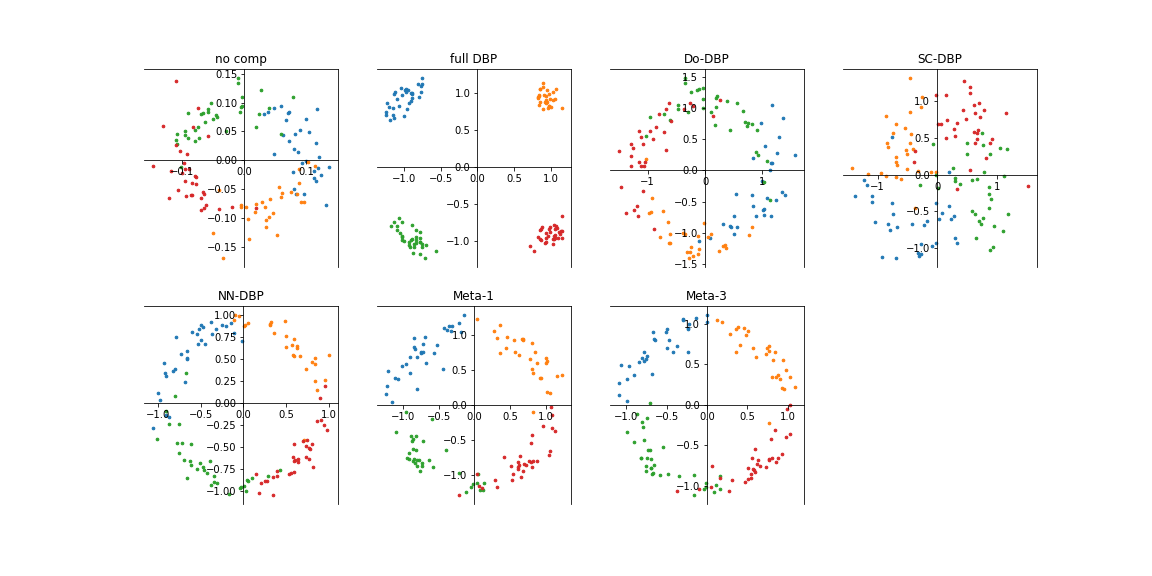
\includegraphics[width=1\linewidth]{img/expriment/W120-D3-P55star.png}
  \end{minipage}
}

\subfigure[test power: 60 mW]{
  \begin{minipage}[t]{0.8\linewidth}
    \centering
    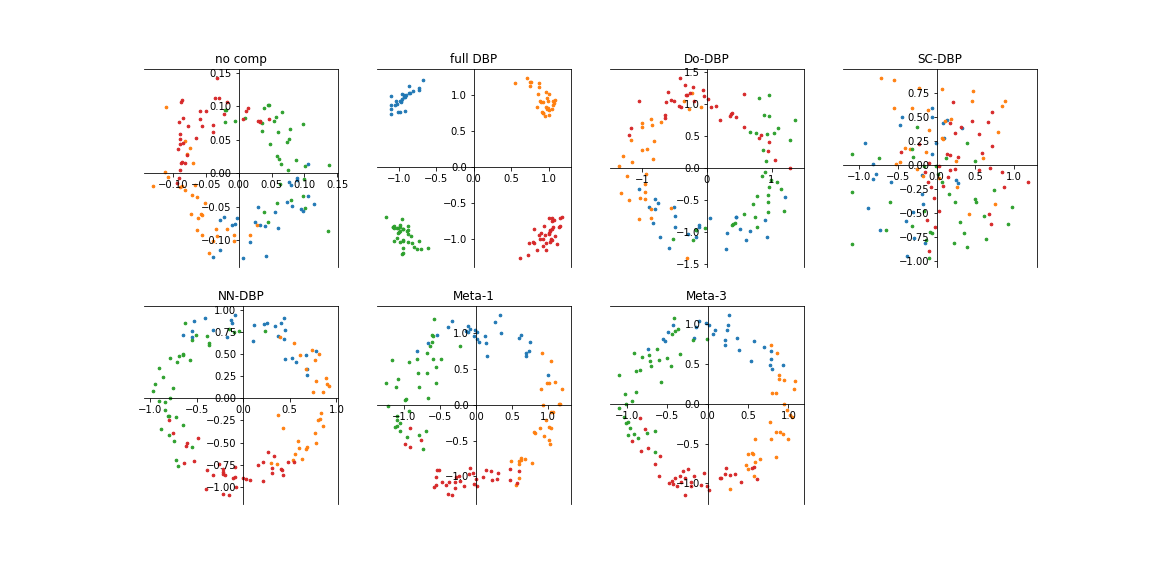
\includegraphics[width=1\linewidth]{img/expriment/W120-D3-P60star.png}
  \end{minipage}
}
\caption{Plot the $\tilde{x}_k^0$. Training with data set B, Test with power: 50[mW],55[mW],60[mW]}
\label{B fig}
\end{figure}

\newpage
\section{Future work}
\begin{enumerate}
\item Improve the Meta-NN structure. Use CNN,RNN etc. Test the boundary of our method.
\item Use the data from physical experiment.(Thank Qiri Fan(author of \cite{fan2020NC}) for provding the data).
\item Consider simulating the optical pulse propagation with Vector Manakov–PMD equation.
$$
\begin{aligned}
\frac{\partial \Psi}{\partial z}=&\left(-\frac{1}{2} \alpha-j \boldsymbol{\beta}_{0}-\boldsymbol{\beta}_{1} \frac{\partial}{\partial t}-j \beta_{2} \frac{1}{2} \frac{\partial^{2}}{\partial t^{2}}\right) \Psi 
&+j \frac{8}{9} \gamma|\boldsymbol{\Psi}|^{2} \boldsymbol{\Psi}+\left[\begin{array}{l}
n_{x}(z, t) \\
n_{y}(z, t)
\end{array}\right]
\end{aligned}
$$
\item Change the system parameter to approach real optical fiber system. In particular, increase 
symbol rate to 60 [GHz]. Increase number of spans to about 10. Change the distributed noise to EDFA noise.
Reduce peak power to about 1[mW]. Increase number channels. The most important thing is to think about how
to pose the problem. Under what circumstances can it be resolved, and under what circumstances will it reach the unsolvable boundary。
\item Improve the structure of the transmitter and receiver, set reasonable down sampling rules, and add some classic adaptive filters and adaptive phase noise estimators (FOE, CPE) to improve
System performance.
\item Considering the calculation limitations of practical applications, balance calculation performance and accuracy improvement.
\end{enumerate}


